\documentclass[11pt]{article}

\usepackage[margin=1in]{geometry}
\usepackage[T1]{fontenc}
\usepackage{lmodern}
\usepackage{microtype}
\usepackage{amsmath,amssymb}
\usepackage{booktabs}
\usepackage{enumitem}
\usepackage{caption}
\usepackage{float}
\usepackage{graphicx}
\usepackage{xcolor}
\usepackage{tikz}
\usetikzlibrary{arrows.meta,positioning,fit,backgrounds}
\usepackage[colorlinks=true,linkcolor=blue!50!black,citecolor=blue!50!black,urlcolor=blue!50!black]{hyperref}

\setlist{itemsep=0pt,topsep=2pt,parsep=0pt}
\usepackage[compact]{titlesec}
\titlespacing*{\section}{0pt}{8pt}{4pt}
\titlespacing*{\paragraph}{0pt}{4pt}{0.8em}
\setlength{\textfloatsep}{8pt plus 2pt}
\setlength{\floatsep}{6pt plus 2pt}
\setlength{\intextsep}{6pt plus 2pt}
\captionsetup{font=small,labelfont=bf}
\newcommand{\taubar}{\bar{\tau}}
\newcommand{\code}[1]{\texttt{\small #1}}

\title{\textbf{Off-Policy GRPO for Online Speculative Decoding}\\[2pt]
\large\emph{MSAI-635 Interim Report}}
\author{
\begin{tabular}{ccc}
Gaurav Prakash & Sanjana Kommareddy & Simran Kharbanda \\
UID: 122250130 & UID: 122099364 & UID: 122283671
\end{tabular}}
\date{}

\begin{document}
\maketitle
\vspace{-2em}

\section{Introduction and Scope}

Speculative decoding lets a small \emph{draft} model propose $K$ tokens that a large \emph{target} model verifies
in one forward pass; verification keeps the longest correct prefix plus one target token, so the output is
exactly the target's. The speed-up depends almost entirely on the mean acceptance length $\taubar$ (accepted
draft tokens per verification step). Our proposal argued that the drafter should be trained \emph{online}, on the
traffic it serves, and proposed replacing the usual forward-KL distillation loss with an off-policy GRPO objective
that rewards accepted length directly.

\paragraph{Change of plan since the proposal.} The published online-training system (Aurora) targets Qwen3-8B on
several 80\,GB GPUs and depends on a CUDA-only stack. We first need a forward-KL baseline that we fully control,
so the project has two phases:
\begin{enumerate}
  \item \textbf{Base-paper reproduction (nearly complete):} online EAGLE-3 draft training, scaled down to
  Qwen3-0.6B and run with PyTorch's MPS backend on Mac laptops. The draft model, loss and data code are reused
  from the paper's release; the serving and orchestration layers are our own.
  \item \textbf{GRPO extension (next):} the off-policy GRPO objective from the proposal, built on the
  reproduction. The system already logs the quantities GRPO needs: per-round accepted length (the reward) and,
  for every round, the served draft version and the trainer's version (the staleness $\Delta$).
\end{enumerate}

\section{Progress So Far}

The reproduction is split into nine work items, each with a concrete ``done when'' criterion
(Table~\ref{tab:progress}). Seven are complete and merged; the online system and its evaluation run end to end.

\begin{table}[t]
\centering\small
\caption{Reproduction work items and their status.}
\label{tab:progress}
\footnotesize\begin{tabular}{@{}p{8.4cm}p{6.0cm}l@{}}
\toprule
Work & Done-when criterion & Status \\
\midrule
Mac environment, device layer (CUDA $\to$ MPS $\to$ CPU), EAGLE-3 code installed without CUDA-only dependencies
  & Draft and EAGLE-3 modules import; parser and vocab tests pass & Done \\
Public datasets (chat, code, math), three request streams, 24K draft-vocab mapping
  & Streams and cached mapping on disk & Done \\
Qwen3-0.6B target with auxiliary hidden-state capture; EAGLE-3 draft and trainer step on MPS
  & Draft overfits one batch in 200 steps; time and memory measured & Done \\
Offline static EAGLE-3 baseline trained on held-in chat data
  & $\taubar$ clearly $>0$ on held-out chat & Done \\
Speculative-decoding server: draft, verify, accept, KV cache, logging, training samples, weight hot-swap
  & Greedy output token-identical to plain decoding on 50 prompts & Done \\
Online loop: sample pool, trainer, versioned weight publish; sync and async; day-0 and with-draft starts
  & $\taubar$ rises over 300 day-0 requests & Done \\
Metrics, latency bench, CSV/summary writer, plots, online losslessness regression test
  & Plots and tables from the run logs & Done \\
\midrule
Controlled experiments: domain shift, ordered stream, sync interval, learning rate, sync vs.\ async
  & Results table and figures & Next \\
Scale check on a CUDA GPU with Qwen3-1.7B/4B & Same code runs on CUDA & Optional \\
\bottomrule
\end{tabular}
\end{table}

\paragraph{Data.} The paper's mixed-domain training data is private, so we built public replacements: 1000
conversations each from ShareGPT (chat), CodeAlpaca-20k (code) and GSM8K (math), filtered to start with a user
turn and to fit in 1024 tokens. From these pools we emit three request streams: \emph{mixed} (3000 requests,
shuffled), \emph{ordered} (3000, grouped by domain) and \emph{domain-shift} (1200: 600 chat, then 300 code, then
300 math). The draft predicts a reduced 24K-token vocabulary (out of Qwen3's 152K), built from assistant-token
frequencies on the mixed stream.

\paragraph{Models.} The target is Qwen3-0.6B (596M parameters), with auxiliary hidden states captured from layers
1, 13 and 24. The EAGLE-3 draft is a single Llama decoder layer (hidden size 1024) fed by a linear fusion of the
three auxiliary states (3072$\to$1024) and the token embedding: 42.4M trainable parameters (24.6M in its 24K-row
output head) plus a frozen 155.6M-parameter embedding copied from the target. Training uses a three-step
test-time-training (TTT) unroll with loss $\sum_i 0.8^i\,\mathcal{L}_i$, where $\mathcal{L}_i$ is the
cross-entropy against the target's soft distribution at unroll step $i$.

\paragraph{Static baseline.} No public EAGLE-3 draft exists for Qwen3-0.6B, so we trained one offline on the chat
pool, holding out its last 100 conversations: AdamW at $10^{-4}$, warmup plus cosine, effective batch 8, fp32
weights, gradient checkpointing, 8 epochs (896 steps, 19 minutes). The 170\,MB checkpoint is published as a
GitHub release with a SHA-256 checksum, so every member starts from identical weights. It is both the
\emph{static} baseline and the starting point for \emph{with-draft} online training.

\paragraph{Inference server.} An HF-transformers draft--verify loop at batch size 1. Each round the draft proposes
$K=3$ guesses and the target scores them in one pass using a \code{DynamicCache} (cropped on rejection), with
greedy (exact argmax match) or speculative-sampling ($\min(1,p/q)$, residual resampling) acceptance. It logs
per-round accepted lengths and draft versions, emits training samples, and can load new draft weights between
requests.

\paragraph{Online loop.} The server's training samples go into a bounded \emph{sample pool} (128 samples, kept on
the CPU); serving blocks when the pool is full rather than dropping samples. A separate \emph{online trainer} owns
its own fp32 copy of the draft and runs the static-baseline recipe on batches from the pool at a constant learning
rate ($10^{-4}$ day-0, $10^{-5}$ with-draft). Every $N$ steps it \emph{publishes} a copy of its weights into a
single pending slot, versioned by its step count; the server applies it before its next request. In \emph{sync}
mode the loop alternates between serving $B$ requests and training $M$ steps. In \emph{async} mode a serving
thread and a training thread run concurrently; because MPS aborts when two threads issue GPU work at once, a FIFO
device lock serialises their GPU calls. Every request records the trainer's version, so staleness $\Delta$ is exact.

\paragraph{Evaluation tooling.} All metrics are recomputed from a run's request and training logs: rolling
$\taubar$, per-position acceptance $\alpha_i$, acceptance rate, tokens/s against target-only decoding, the
estimated speed-up $(1+\taubar)/(1+Kc)$, staleness and the loss curve. A latency bench measures $c$, the cost of
one draft step relative to one target step. Output is CSV, JSON and plots. The repository has 68 tests,
including losslessness under live weight swaps in sync and async modes.

\section{Notional Architecture}

Figure~\ref{fig:arch} shows the system as built. The GRPO extension changes only the trainer's loss and adds tree
drafting to the drafter, to produce groups of rollouts; everything else is reused. Compared with the paper's
deployment, the multi-GPU serving engine, transfer store, cluster scheduler and sharded trainer are replaced by
an in-process pool, a single-device trainer and an in-memory publish slot; the target shrinks from 8B to 0.6B,
the draft vocabulary from 32K to 24K, and $K$ and the TTT length from 5 to 3.

\begin{figure}[t]
\centering
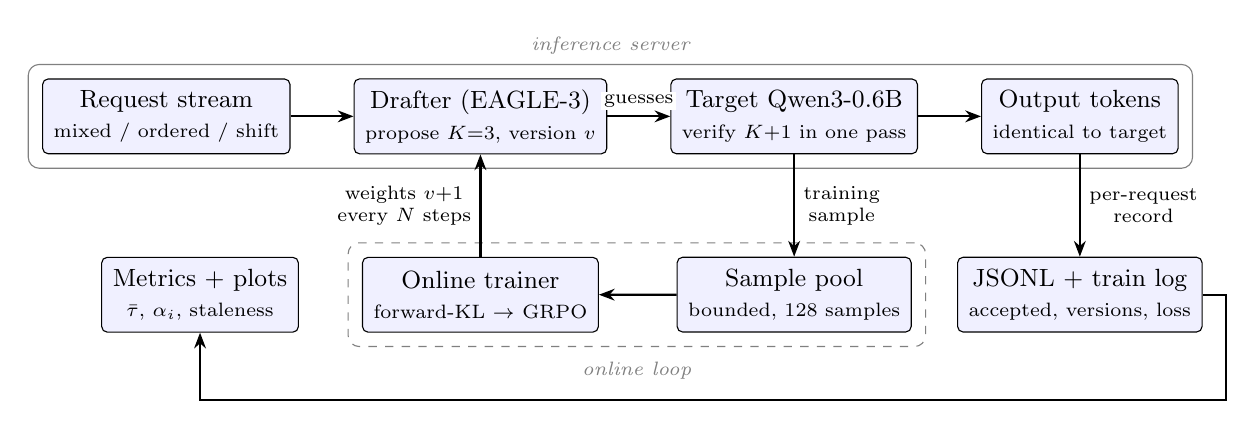
\begin{tikzpicture}[
  font=\small,
  box/.style={draw, rounded corners=2pt, align=center, minimum height=0.95cm, inner sep=4pt, fill=blue!6},
  arr/.style={-{Stealth[length=2mm]}, thick},
  lab/.style={font=\scriptsize, align=center, fill=white, inner sep=1pt}
]
\node[box] (stream) {Request stream\\{\scriptsize mixed / ordered / shift}};
\node[box, right=0.8cm of stream] (draft) {Drafter (EAGLE-3)\\{\scriptsize propose $K{=}3$, version $v$}};
\node[box, right=0.8cm of draft] (target) {Target Qwen3-0.6B\\{\scriptsize verify $K{+}1$ in one pass}};
\node[box, right=0.8cm of target] (out) {Output tokens\\{\scriptsize identical to target}};
\node[box, below=1.3cm of draft] (trainer) {Online trainer\\{\scriptsize forward-KL $\to$ GRPO}};
\node[box, below=1.3cm of target] (pool) {Sample pool\\{\scriptsize bounded, 128 samples}};
\node[box, below=1.3cm of out] (log) {JSONL + train log\\{\scriptsize accepted, versions, loss}};
\node[box, left=0.8cm of trainer] (metrics) {Metrics + plots\\{\scriptsize $\taubar$, $\alpha_i$, staleness}};

\draw[arr] (stream) -- (draft);
\draw[arr] (draft) -- node[lab, above=2pt] {guesses} (target);
\draw[arr] (target) -- (out);
\draw[arr] (target.south) -- node[lab, right=2pt] {training\\sample} (pool.north);
\draw[arr] (pool) -- (trainer);
\draw[arr] (trainer.north) -- node[lab, left=2pt] {weights $v{+}1$\\every $N$ steps} (draft.south);
\draw[arr] (out.south) -- node[lab, right=2pt] {per-request\\record} (log.north);
\draw[arr] (log.east) -- ++(0.3,0) |- ([yshift=-0.85cm]metrics.south) -- (metrics.south);

\begin{scope}[on background layer]
  \node[draw=gray, rounded corners, fit=(stream)(draft)(target)(out), inner sep=5pt,
        label={[font=\scriptsize\itshape, gray]above:inference server}] {};
  \node[draw=gray, dashed, rounded corners, fit=(trainer)(pool), inner sep=5pt,
        label={[font=\scriptsize\itshape, gray, yshift=-2pt]below:online loop}] {};
\end{scope}
\end{tikzpicture}
\caption{System architecture (all components implemented). The trainer's objective is forward KL in the
reproduction and off-policy GRPO in the extension.}
\label{fig:arch}
\end{figure}

\section{Frameworks and Libraries}

\begin{itemize}
  \item \textbf{PyTorch 2.14} on the MPS backend (Apple GPU), eager mode with SDPA attention; tests also run with
  CPU fallback disabled. Python threads for the async loop.
  \item \textbf{Hugging Face} \code{transformers} 4.57.1 (target model, \code{DynamicCache}, chat templates),
  \code{datasets} and \code{huggingface\_hub} (ShareGPT, CodeAlpaca, GSM8K), \code{accelerate}, \code{safetensors}.
  \item \textbf{Paper's EAGLE-3 code} (installed without its CUDA-only dependencies): draft model, TTT wrapper,
  target-feature hooks, vocab mapping, conversation parser.
  \item \textbf{Tooling:} \code{uv} with Python 3.12, \code{pytest}, \code{matplotlib}, a Docker CPU image, a cloud
  CUDA notebook for an independent GPU check, GitHub releases for checkpoints and one issue / PR per work item.
\end{itemize}

\section{Baselines and State of the Art}
\label{sec:baselines}

\paragraph{Lineage.} Speculative decoding with lossless verification (Leviathan et al.; Chen et al., 2023) uses a
separate small LM as the draft. Medusa adds parallel decoding heads to the target. The EAGLE family drafts from
the target's own hidden states; EAGLE-2 adds dynamic draft trees, and EAGLE-3 fuses low-, mid- and high-level
features and trains with a test-time-training unroll. EAGLE-3 is the state-of-the-art drafter and the one we use.
Online Speculative Decoding first proposed distilling the draft on live traffic, and Aurora turns this into a
unified training--serving system with asynchronous weight hot-swap; this is the method we reproduce. GRPO is the
critic-free RL objective our extension adapts.

\paragraph{Systems we compare.} All are evaluated on the same streams and decoding settings: (1)~\textbf{target
only}, the speed-up reference; (2)~\textbf{static EAGLE-3}, the frozen offline draft (``train offline, then
deploy''); (3)~\textbf{online day-0}, online forward-KL training from a random draft; (4)~\textbf{online
with-draft}, online forward-KL training from the static draft; (5)~\textbf{ours}, off-policy GRPO with a forward-KL
anchor, with the ablations from the proposal (synchronous on-policy GRPO, $\Delta=0$; group size $G$; KL weight
$\beta$; clipping and truncation thresholds; reward shaping).

\paragraph{Planned experiments.} Day-0 online training against target-only on the mixed stream (done, below);
static vs.\ with-draft under the chat$\to$code$\to$math domain shift, measured as the area under the
rolling-$\taubar$ curve after each shift; the same on the ordered stream; and sensitivity to the sync interval
$N\in\{5,20,50\}$, the learning rate, and sync vs.\ async training. The headline metric is $\taubar$, which does not
depend on hardware; we also report $\alpha_i$, measured and estimated speed-up, and the staleness distribution.

\section{Evaluation Results (Prototype)}
\label{sec:results}

All runs use MPS on Mac laptops, greedy decoding, $K=3$ guesses per round and up to 128 new tokens. We report two
numbers per run: the \textbf{token acceptance} $\taubar$ (draft guesses accepted per round, out of 3; papers often
report $1+\taubar$, tokens per target pass) and the \textbf{speed-up} over target-only decoding of the same
requests. Table~\ref{tab:main} summarises every draft we have run.

\begin{table}[t]
\centering\small
\caption{Main results. Speed-up is measured against target-only decoding of the same requests in the same run.
Wherever checked (450 requests), output was token-identical to target-only decoding.}
\label{tab:main}
\setlength{\tabcolsep}{5pt}
\begin{tabular}{@{}llccc@{}}
\toprule
Draft & Requests & $\taubar$ (of 3) & Tokens / target pass & Speed-up \\
\midrule
Untrained (lower bound) & 50 mixed & 0.00 & 1.00 & 0.56$\times$ \\
Overfit to the answers (upper bound) & 50 mixed & 2.60 & 3.60 & 2.0$\times$ \\
\midrule
Static, 2 epochs offline & 100 held-out chat & 0.18 & 1.18 & 0.53$\times$ \\
\textbf{Static, 8 epochs offline (baseline)} & 100 held-out chat & \textbf{0.31} & \textbf{1.31} & \textbf{0.59$\times$} \\
\midrule
Online day-0, whole run & 300 mixed & 0.15 & 1.15 & 0.53$\times$ \\
\textbf{Online day-0, last 50 requests} & 50 mixed & \textbf{0.25} & \textbf{1.25} & -- \\
Online with-draft (short test) & 20 mixed & $\approx$0.26 & 1.26 & -- \\
\bottomrule
\end{tabular}
\end{table}

\begin{figure}[t]
\centering
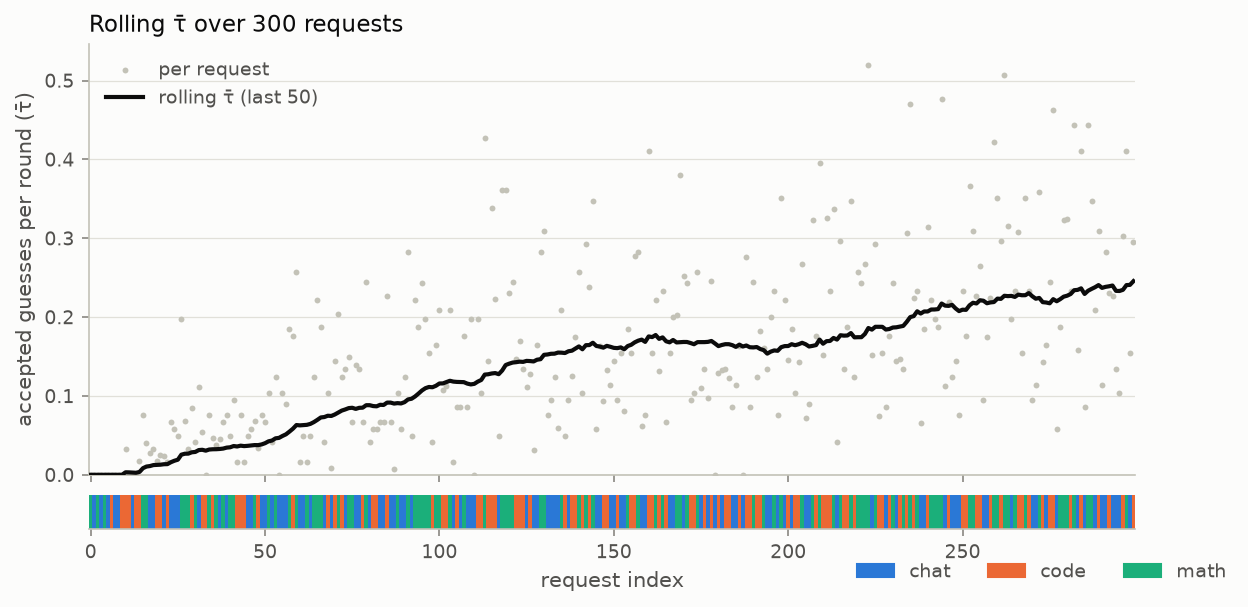
\includegraphics[width=0.62\linewidth]{figures/rolling_tau.png}
\caption{Online day-0 run: token acceptance per request (dots) and averaged over the last 50 requests (line),
with each request's domain underneath.}
\label{fig:rolling}
\end{figure}

\paragraph{What the results say.}
\begin{enumerate}
  \item \textbf{The output is always exact.} Speculative output matched target-only decoding on all 450 checked
  requests, including 300 during which the online trainer replaced the draft's weights 30 times.
  \item \textbf{Offline training works.} Eight epochs on 900 chat conversations take acceptance from 0 to 0.31.
  \item \textbf{Online training works from scratch.} Starting from a random draft, acceptance rises from 0.04 to
  0.25 within 300 requests (Figure~\ref{fig:rolling}) and is still rising, reaching 80\% of the static draft
  with a sixth of its training steps. It learns fastest on math (0.32 by the end), then code (0.23), then chat
  (0.13). Starting online training from the static draft skips this warm-up: it is at 0.26 from the first request.
  \item \textbf{No speed-up yet.} Each round costs about 2.2 target-only steps but produces only $1+\taubar$
  tokens, so the draft must average about 1.2 accepted guesses per round to break even; ours average 0.15--0.31,
  almost all at the first guess. The upper-bound row shows the server itself can reach 2$\times$ when the draft
  guesses well, so the bottleneck is draft quality.
  \item \textbf{Staleness is small.} The served draft lags the trainer by 2 steps on average (at most 4), with no
  effect on correctness. Precision does not change acceptance (fp32 and bf16 runs give the same curve).
\end{enumerate}

\paragraph{Relation to published results.} Published EAGLE-2/3 drafts on 8B--70B targets with tree drafting
report roughly 4--6 tokens per target pass and 3--6$\times$ speed-ups; classic speculative decoding and Medusa
report about 2--3$\times$. We are at 1.3 tokens per pass and below 1$\times$. The gap is expected: our drafts have
seen thousands rather than hundreds of thousands of conversations, we draft a single chain of 3 instead of a
tree, a 0.6B target makes the draft relatively expensive (one draft step costs a tenth of a target step), and MPS
at batch size 1 lacks production kernels and batching. We therefore compare systems \emph{against each other} on
the same setup, with acceptance as the headline metric.

\section{Issues Faced}

\paragraph{Solved.}
\begin{itemize}
  \item \textbf{Compute and CUDA-only stack:} scaled down to Qwen3-0.6B on MPS with our own server, pool,
  trainer and publish slot, while reusing the published draft, loss and data code unchanged.
  \item \textbf{No public draft, private data:} trained our own EAGLE-3 draft on public data; ShareGPT filters
  drop 939 threads that start mid-conversation and 613 longer than 1024 tokens.
  \item \textbf{Draft-vocab coverage:} 16K covered only 97.6\% of assistant tokens (others can never be drafted);
  24K covers 0.993 / 0.995 / 0.998 (chat / code / math) for 8.2M more parameters.
  \item \textbf{Memory:} 4$\times$1K-token batches needed 9.9\,GB (draft logits $\times$ 3 TTT steps); batch 2 with
  gradient checkpointing trains in 2.4\,GB, and the whole online loop peaks at 7.5\,GB, so it fits a 16\,GB laptop.
  \item \textbf{Precision:} pure-bf16 AdamW lost 2--3 accuracy points (small updates round away), so the trainer
  always keeps fp32 weights and checkpoints reload in their trained dtype. In bf16, a 4-token verify pass rounds
  differently from 4 single steps and can flip near-ties, so losslessness checks run in fp32 (450/450 pass).
  \item \textbf{Threads on MPS:} MPS aborts when two threads use the GPU at once; async mode serialises GPU calls
  with a FIFO device lock.
  \item \textbf{Sharing checkpoints:} the static draft is a GitHub release with a SHA-256 checksum.
\end{itemize}

\paragraph{Open.}
\begin{itemize}
  \item \textbf{No wall-clock speed-up yet.} Levers: higher $\taubar$ (more online training, GRPO), a draft KV
  cache, and tree drafting.
  \item \textbf{Train/test overlap in the streams.} The 600 chat requests of the domain-shift stream, and 900 of
  the 1000 chat requests in the mixed stream, were static-baseline training prompts. This does not affect day-0
  runs, but before the domain-shift comparisons we must rebuild the chat segments from held-out conversations or
  report on unseen requests only.
  \item \textbf{Single-device asynchrony.} With the device lock, ``async'' on one GPU interleaves rather than
  overlaps serving and training, so staleness is real but smaller than with separate serving and training GPUs.
  \item \textbf{Hardware variance.} A fanless laptop slowed $\sim$12\% over an hour (the speed ratio held at
  0.53--0.54), so we only compare speeds within a run.
  \item \textbf{GRPO prerequisites.} Groups of rollouts need tree drafting (top-$k>1$), which is not yet
  implemented, and $K=3$ gives a shorter reward range than $K=5$.
\end{itemize}

\section{Next Steps}

\begin{enumerate}
  \item \textbf{With-draft run:} 300 mixed requests from the released static draft, with the same settings as
  the day-0 run, for a direct comparison.
  \item \textbf{Controlled experiments}, after removing the stream overlap: static vs.\ day-0 vs.\ with-draft on
  the domain-shift and ordered streams, and sweeps over $N$, learning rate and sync vs.\ async.
  \item \textbf{GRPO extension:} tree drafting for groups; reward $R(a)=L(a)-\lambda\kappa(K-L(a))$ from the
  logged accepted lengths; the off-policy objective with truncated importance weights and the forward-KL
  anchor, using the logged staleness; and comparison against systems 2--4 above.
  \item \textbf{Scale check (optional):} the same code on a CUDA GPU with a larger target, to check that the
  trends carry over.
\end{enumerate}

\end{document}
